\documentclass[12pt]{article}
\usepackage[svgnames,x11names,table]{xcolor}
\usepackage{hyperref}
\usepackage{graphicx}
\usepackage{parskip}
\usepackage{float}
\usepackage{amsmath}
\usepackage{amssymb}
\usepackage{enumitem}
\usepackage[thicklines]{cancel}

\hypersetup{
    colorlinks,
    citecolor=blue,
    filecolor=black,
    linkcolor=black,
    urlcolor=RoyalBlue4,
}

\title{PEU 218 Assignment 2}
\author{Mohamed Hussien El-Deeb (201900052)}
\date{\today}

\begin{document}

\maketitle
\tableofcontents
\hypersetup{linkcolor=RoyalBlue4}

\newpage
\section{Question 1}

\subsection{Problem}

Evaluate
\[
    \int_C \left(2y x^2 - 4x\right) d r
\]

Where \(C\) is lower half of the circle centered at the origin of radius 3 with clockwise
rotation.

\subsection{Solution}

\[x = 3 \cos(\theta)\]

\[y = 3 \sin(\theta)\]

\[
    \vec{r} = \left\langle x, y\right\rangle =
    \left\langle 3 \cos(\theta), 3 \sin(\theta)\right\rangle
\]

\[
    d \vec{r} = 3 \left\langle -\sin(\theta), \cos(\theta)\right\rangle d\theta
\]

\[
    d r = 3 d \theta
\]



The limits of integration are \(\theta = \pi \) to \(\theta = 0\).

\[
    \int_C \left(2y x^2 - 4x\right) d r
    = 18 \int_{\pi}^{0} \left(9 \sin(\theta) \cos^2(\theta) - 2 \cos(\theta)\right) d \theta
\]

\[
    = 18 {\left[3 \cos^3(\theta) + 2 \sin(\theta)\right]}_{0}^{\pi}
    = -108
\]

\newpage
\section{Question 2}

\subsection{Problem}

Evaluate \(\int_C \vec{F} \cdot d \vec{r}\), where
\(\vec{F}=\left\langle y, 3y^3 - x, z\right\rangle \) and the path \(C\) is defined by
\(C(t) = \left\langle t, t^n, 0\right\rangle, 0 \leq t \leq 1\) where \(n = 1, 2, 3, .. \)

\subsection{Solution}

\[
    \vec{r} = \left\langle t, t^n, 0\right\rangle
\]

\[
    d \vec{r} = \left\langle 1, n t^{n - 1}, 0\right\rangle d t
\]

\[
    \vec{F} = \left\langle t^n, 3t^{3n} - t, 0\right\rangle
\]

\[
    \vec{F} \cdot d \vec{r} = 3 n t^{4n - 1} + (1 - n) t^n d t
\]

\[
    \int_{0}^{1} \left(3 n t^{4n - 1} + (1 - n) t^n\right) d t
\]

\[
    = {\left[\frac{3}{4} t^{4n} + \frac{1 - n}{1 + n} t^{n + 1}\right]}_{0}^{1}
    = \frac{3}{4} + \frac{1 - n}{1 + n}
\]

\newpage
\section{Question 3}

\subsection{Problem}

Evaluate \(\int_C \vec{F} \cdot d \vec{r}\), where \(\vec{F} = \langle xy, 1 + 3y, 0\rangle \) and
\(C\) is the line segment from \((0, -4)\) to \((-2, -4)\) followed by portion of \(y = -x^2\)
from \(x = -2\) to \(x = 2\) which is in turn followed by the line segment from \((2, -4)\)
to \((5, 1)\).

\subsection{Solution}

I will reduce the dimension of the problem to 2D since \(\vec{F}\) is the
only 3D vector and its z component is 0.

\begin{figure}[H]
    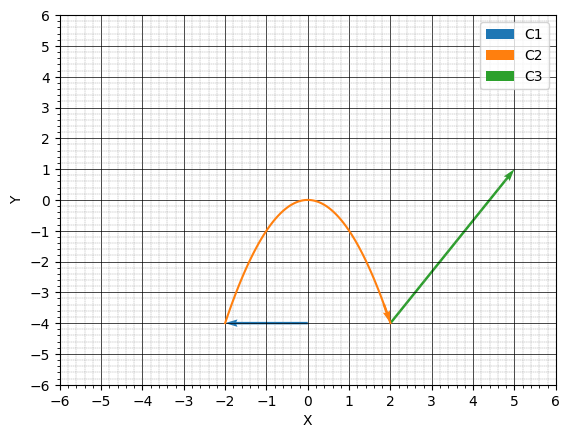
\includegraphics[width=\linewidth]{Q3.png}
    \caption{Path equations for the three contours.\cite{El-Deeb_PEU-218_Assignments_py}}\label{fig:Q3}
\end{figure}

\[
    \vec{F} = \left\langle xy, 1 + 3y\right\rangle
\]

\[
    C1 = \left\langle -2t, -4\right\rangle, \quad t = [0, 1]
\]

\[
    \vec{F}_1 = \left\langle 8t, -11 \right\rangle
\]

\[
    d \vec{r}_1 = \left\langle -2, 0\right\rangle d t
\]

\[
    C2 = \left\langle t, -t^2\right\rangle, \quad t = [-2, 2]
\]

\[
    \vec{F}_2 = \left\langle -t^3, 1 - 3t^2\right\rangle
\]

\[
    d \vec{r}_2 = \left\langle 1, -2t\right\rangle d t
\]

\[
    C3 = \left\langle 3t + 2, 5t -4\right\rangle, \quad t = [0, 1]
\]

\[
    \vec{F}_3 = \left\langle 15t^2 - 2t - 8, 15t - 11\right\rangle
\]

\[
    d \vec{r}_3 = \left\langle 3, 5\right\rangle d t
\]

\[
    \int_C \vec{F} \cdot d \vec{r}
    = \int_{C1} \vec{F}_1 \cdot d \vec{r}_1
    + \int_{C2} \vec{F}_2 \cdot d \vec{r}_2
    + \int_{C3} \vec{F}_3 \cdot d \vec{r}_3
\]

\[
    = \int_{-2}^{2} \left(5t^3 - 2t\right) d t
    + \int_{0}^{1} \left(45t^2 + 53t - 79\right) d t
\]

\[
    = \left[\frac{5}{4} t^4 - t^2\right]_{-2}^{2}
    + {\left[15t^3 + \frac{53}{2} t^2 - 79t\right]}_{0}^{1}
    = -37.5
\]

\newpage
\section{Question 4}

\subsection{Problem}

Evaluate \(\iint_S 2y\ dS\) where \(S\) is the portion \(y^2 + z^2 = 4\) between \(x = 0\)
and \(x = 3 - z\).

\subsection{Solution}



\newpage
\section{Question 5}

\subsection{Problem}

Let the temperature of a point in space be given by \(T(x, y, z)= 3x^2 + 3z^2\).
Compute the heat flux across the surface \(x^2 + z^2 = 2, 0 \leq y \leq 2\), if \(k = 1\).
(Give a physical explanation to justify the sign of your result?)

\subsection{Solution}



\newpage
\section{Question 6}

\subsection{Problem}

Evaluate \(\iint_S \vec{F} \cdot d S\) where
\(\vec{F} = y \hat{\imath} + 2x \hat{\jmath} + (z - 8) \hat{k}\) and \(S\) is the surface of the
solid bounded by \(4x + 2y + z = 8, z = 0, y = 0\) and \(x = 0\) with the positive orientation.
Note that all four surfaces of the solid are included in \(S\).

\subsection{Solution}



\newpage
\bibliographystyle{plain}
\bibliography{references}
\nocite{El-Deeb_PEU-218_Assignments}

\end{document}